

\tikzset{every picture/.style={line width=0.75pt}} %set default line width to 0.75pt        

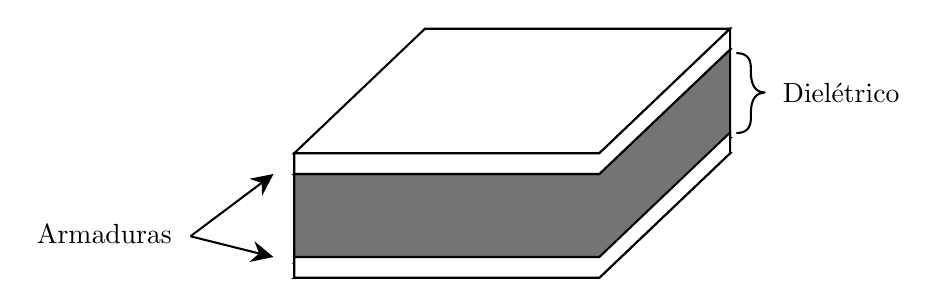
\begin{tikzpicture}[x=0.75pt,y=0.75pt,yscale=-1,xscale=1]
%uncomment if require: \path (0,300); %set diagram left start at 0, and has height of 300

%Shape: Parallelogram [id:dp8548990547558715] 
\draw  [color={rgb, 255:red, 0; green, 0; blue, 0 }  ,draw opacity=1 ] (273,150) -- (420,150) -- (357,210) -- (210,210) -- cycle ;
%Shape: Parallelogram [id:dp2597151772975901] 
\draw  [color={rgb, 255:red, 0; green, 0; blue, 0 }  ,draw opacity=1 ] (273,100) -- (420,100) -- (357,160) -- (210,160) -- cycle ;
%Shape: Parallelogram [id:dp6375542356566128] 
\draw   (273,142.73) -- (420,142.73) -- (357,202.73) -- (210,202.73) -- cycle ;
%Shape: Polygon [id:ds45164816369455796] 
\draw  [fill={rgb, 255:red, 116; green, 116; blue, 116 }  ,fill opacity=1 ] (420,100) -- (420,142.73) -- (357,202.73) -- (210,202.73) -- (210,160) -- (357,160) -- cycle ;
%Shape: Parallelogram [id:dp32528907626678527] 
\draw  [color={rgb, 255:red, 0; green, 0; blue, 0 }  ,draw opacity=1 ][fill={rgb, 255:red, 255; green, 255; blue, 255 }  ,fill opacity=1 ] (273,90) -- (420,90) -- (357,150) -- (210,150) -- cycle ;
%Shape: Polygon [id:ds7050436133230993] 
\draw  [fill={rgb, 255:red, 255; green, 255; blue, 255 }  ,fill opacity=1 ] (420,90) -- (420,100) -- (357,160) -- (210,160) -- (210,150) -- (357,150) -- cycle ;
%Shape: Polygon [id:ds6883853167125011] 
\draw  [fill={rgb, 255:red, 255; green, 255; blue, 255 }  ,fill opacity=1 ] (420,140) -- (420,150) -- (357,210) -- (210,210) -- (210,200) -- (357,200) -- cycle ;
%Shape: Brace [id:dp9390925081485437] 
\draw   (423,140.25) .. controls (427.67,140.25) and (430,137.92) .. (430,133.25) -- (430,130.75) .. controls (430,124.08) and (432.33,120.75) .. (437,120.75) .. controls (432.33,120.75) and (430,117.42) .. (430,110.75)(430,113.75) -- (430,108.75) .. controls (430,104.08) and (427.67,101.75) .. (423,101.75) ;
%Straight Lines [id:da5772252064441987] 
\draw    (160,190) -- (197.6,161.8) ;
\draw [shift={(200,160)}, rotate = 503.13] [fill={rgb, 255:red, 0; green, 0; blue, 0 }  ][line width=0.08]  [draw opacity=0] (10.72,-5.15) -- (0,0) -- (10.72,5.15) -- (7.12,0) -- cycle    ;

%Straight Lines [id:da1261577538308405] 
\draw    (160,190) -- (197.09,199.27) ;
\draw [shift={(200,200)}, rotate = 194.04] [fill={rgb, 255:red, 0; green, 0; blue, 0 }  ][line width=0.08]  [draw opacity=0] (10.72,-5.15) -- (0,0) -- (10.72,5.15) -- (7.12,0) -- cycle    ;


% Text Node
\draw (473.5,121) node  [align=left] {Dielétrico};
% Text Node
\draw (118.5,189) node  [align=left] {Armaduras};


\end{tikzpicture}